\documentclass{beamer}

%Colorir Ruby
\usepackage{minted}

% Codificação UTF-8
\usepackage[brazilian]{babel}
\usepackage[utf8]{inputenc}

% Imagens
\usepackage{graphicx}

% Tabela teszte
\usepackage{xcolor,colortbl}

\definecolor{fabsoft-one}{RGB}{48,26,193}
\definecolor{fabsoft-two}{RGB}{76,49,255}
\definecolor{fabsoft-three}{RGB}{108,85,255}
%TESTE DE COMENTARIO...
\definecolor{gray-one}{RGB}{226,226,226}
\definecolor{gray-two}{RGB}{174,174,174}
\definecolor{header-color}{RGB}{50,50,50}
\definecolor{gold}{HTML}{FDD017}

%\usetheme{Madrid}
\usetheme{CambridgeUS}
%\definecolor{kugreen}{RGB}{50,93,61}
%\definecolor{kugreenlys}{RGB}{132,158,139}
%\definecolor{kugreenlyslys}{RGB}{173,190,177}
%\definecolor{kugreenlyslyslys}{RGB}{214,223,216}


%\definecolor{deep sky blue}{HTML}{3BB9FF}
%\definecolor{light sky blue}{HTML}{82CAFA}
%
%\definecolor{mybackground}{HTML}{82CAFA}
%\definecolor{myforeground}{HTML}{0000A0}

%\setbeamercolor{normal text}{fg=gold,bg=gold}
%\setbeamercolor{title text}{fg=gold}
%\setbeamercolor{example text}{fg=gold}
\setbeamercolor{title}{fg=fabsoft-one}
\setbeamercolor{frametitle}{fg=fabsoft-one}


%\setbeamercolor{background canvas}{fg=myforeground, bg=white}
%\setbeamercolor{background}{fg=myforeground, bg=mybackground}
%
\setbeamercolor{palette primary}{fg=fabsoft-one}
\setbeamercolor{palette secondary}{fg=fabsoft-one}
\setbeamercolor{palette tertiary}{fg=white, bg=fabsoft-one}

%\setbeamercovered{transparent}



%\usecolortheme[named=kugreen]{structure}

\clearpage

\title{Banco de Dados e Relacionamento}


\subtitle{Rais - Dia 4}

\author[Felipe e Akme-re]{~Felipe Fernandes \and ~Akme-re Almeida}

\institute[Fabsoft] % (optional, but mostly needed)
{}

\date{}

\AtBeginSubsection[]
{
  \begin{frame}<beamer>{Outline}
    \tableofcontents[currentsection,currentsubsection]
  \end{frame}
}

% Let's get started
\begin{document}

\begin{frame}

  \titlepage
  
\end{frame}

\begin{frame}{Agenda}
  \tableofcontents
  % You might wish to add the option [pausesections]
\end{frame}
\begin{frame}[fragile]

\frametitle{Banco de Dados - Conceito}
\section{Banco de Dados}

%\subsection{Conceito}
\begin{block}{\LARGE Conceito}
	\begin{itemize}
		\item \LARGE Coleção de dados armazenados em uma maquina.
		\item \LARGE Base que pode ser acessada por softwares para consultas e atualizações.
	\end{itemize}
\end{block}

%\begin{minted}[linenos,xleftmargin=50]{rb}
%  	def lol
%  		 "hello world"
%  	end
%  	
%  	:sym
%  \end{minted}
\end{frame}

\section{Exemplos}
\begin{frame}[fragile]{Banco de Dados}{Exemplos}
	\begin{columns}
		\begin{column}{0.5\textwidth}
			\begin{figure}
				\begin{minipage}{\columnwidth}
					
\includegraphics[scale=0.5]{images/pg}
				\end{minipage}
				\begin{minipage}{\columnwidth}
					
\includegraphics[scale=1]{images/mysql}
				\end{minipage}
			\end{figure}
		\end{column}
	
		\begin{column}{0.5\textwidth}
			\begin{figure}
				\begin{minipage}{\columnwidth}
					
\includegraphics[scale=0.7]{images/oracle}
				\end{minipage}
				\begin{minipage}{\columnwidth}
					
\includegraphics[scale=0.5]{images/sqlite}
				\end{minipage}
			\end{figure}
		\end{column}
	\end{columns}		
\end{frame}

\section{Ferramenta - SQLiteman}
\begin{frame}[fragile]{Ferramenta}{SQLiteman - Ferramenta gráfica para gerenciar o Banco}
	\begin{figure}
		\begin{minipage}{\columnwidth}
			\centering
				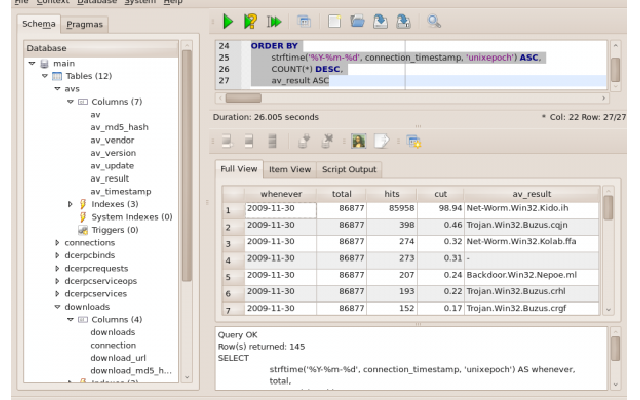
\includegraphics[scale=0.4]{images/sqliteman}
		\end{minipage}
	\end{figure}
\end{frame}
%\subsection{Second Subsection}

% You can reveal the parts of a slide one at a time
% with the \pause command:
\begin{frame}[fragile]{SQLite 3}{Default Rails}
	\begin{itemize}  \itemsep 2em
		\item{ \LARGE Banco de Dados Simples.}
		\item{ \LARGE Apenas para Estudo.}
		\item{ \LARGE Não deve ser usado em projetos robustos.}
		\item{ \LARGE Banco de dados localizado em um unico arquivo.}
								
	\end{itemize}
\end{frame}
%\section{Second Main Section}

%\subsection{Another Subsection}

\begin{frame}{Banco de Dados}{Conceitos Iniciais}
	\begin{itemize} 
		\item{
			\LARGE Bancos Possuem o que?
			\begin{itemize} \itemsep 2em
				\item{ \Large Usuários - Autenticação}
				\item{ \Large Schemas - Organização}
				\item{ \Large Tabelas - Armazenamento}
			\end{itemize}
		}
	\end{itemize}
\end{frame}

\section{Tabelas}
\begin{frame}{SQLite}{Tabela}
	\begin{itemize} 
		\item{
			\LARGE Tabelas
			\begin{itemize} \itemsep 2em
				\item{ \Large Estruturas de armazenamento para os dados.}
				\item{ \Large Schemas - Organização.}
				\item{ \Large Tabelas - Armazenamento.}
			\end{itemize}
		}
	\end{itemize}
\end{frame}
% Placing a * after \section means it will not show in the
% outline or table of contents.
%\section*{Summary}

\begin{frame}{Tabela}
	\begin{center}
		\begin{table}
			\LARGE
			\caption{\label{label}\Large Dividas.}
			\begin{tabular}{ c | l }
					\hline
					\hline
					\hline					
					\rowcolor{header-color} \color{white}\textbf{CONTA}  & \color{white}\textbf{VALOR} \\
					\hline
					Luz & 100.50 \\
					\hline
					Agua & 50.55 \\
					\hline
					Telefone & 45.50 \\
					\hline
					\hline
			\end{tabular}% Tabulação
		\end{table}
	\end{center}
\end{frame}



% All of the following is optional and typically not needed. 
%\appendix
\section<presentation>*{\appendixname}
\subsection<presentation>*{For Further Reading}

\begin{frame}{Index e Chave Primária}
	\begin{center}
		\begin{table}
			\LARGE
			\caption{\label{label}\Large Dividas.}
			\begin{tabular}{ >{\columncolor[gray]{0.8}}c | l | c}
					\hline
					\hline
					\hline					
					\rowcolor{header-color} \color{white}\textbf{ID} &  \color{white}\textbf{CONTA}  & \color{white}\textbf{VALOR} \\
					\hline
					1 & Luz & 100.50 \\
					\hline
					2 & Agua & 50.55 \\
					\hline
					3 & Telefone & 45.50 \\
					\hline
					\hline
			\end{tabular}% Tabulação
		\end{table}
	\end{center}
\end{frame}

\begin{frame}{Chave Estrangeira}
	\begin{block}{\LARGE Chave Estrangeira - Conceito}
		\begin{itemize}
			\item \LARGE Index Especial que liga duas Tabelas para melhor aproveitamento
		\end{itemize}
	\end{block}
\end{frame}

\section{Cardinalidade}

\begin{frame}{Relacionamentos}{Tipos}
	\begin{itemize} \itemsep 2em
		\item{ \LARGE 1 x 1 }
		\item{ \LARGE 1 x N }
		\item{ \LARGE N x N }
	\end{itemize}
\end{frame}

\begin{frame}{Cardinalidade}{1 e 1}
	\begin{center}
%		\begin{table}
%			\Large
%			\caption{\label{label}\Large Pessoas.}
			\begin{tabular}{ c | l | c}
				\hline
				\hline
				\hline					
				\rowcolor{header-color} \color{white}\textbf{ID} &  \color{white}\textbf{NOME}  & \color{white}\textbf{NASCIMENTO} \\
				\hline
				1 & Rodrigo Andrade Silva & 01/09/1994 \\
				\hline
				2 & Felipe Almeida Zamora & 05/10/1990 \\
				\hline
				\hline
			\end{tabular}% Tabulação
%		\end{table}
	\end{center}
		
	\begin{center}
%		\begin{table}
%			\Large
%			\caption{\label{label}\Large Documentos.}
			\begin{tabular}{ l | l | l | >{\columncolor[gray]{0.8}}l }
				\hline
				\hline
				\hline					
				\rowcolor{header-color} \color{white}\textbf{ID} &  \color{white}\textbf{IDENTIDADE}  & \color{white}\textbf{CPF} &  \color{white}\textbf{PES-ID} \\
				\hline
				55 & 55997-65  & 555.999.777 & 2\\ 
				\hline
				56 &  56587-65 & 544.455.545 & 1\\
				\hline
				\hline
			\end{tabular}% Tabulação
%		\end{table}				
	\end{center}

\end{frame}

\begin{frame}{Cardinalidade}{1 e 1}
	\begin{center}
%		\begin{table}
%			\Large
%			\caption{\label{label}Pessoas.}
			\begin{tabular}{ l | l | l |  >{\columncolor[gray]{0.8}}l}
				\hline
				\hline
				\hline					
				\rowcolor{header-color} \color{white}\textbf{ID} & \color{white}\textbf{NOME}  & \color{white}\textbf{NASCIMENTO} & \color{white}\textbf{DOC-ID} \\
				\hline
				1 & Rodrigo Andrade Silva & 01/09/1994 & 56\\
				\hline
				2 & Felipe Almeida Zamora & 05/10/1990 & 55\\
				\hline
				\hline
			\end{tabular}% Tabulação
%		\end{table}
	\end{center}
		
	\begin{center}
%		\begin{table}
%			\Large
%			\caption{\label{label}\large Documentos.}
			\begin{tabular}{ l | l | l }
				\hline
				\hline
				\hline					
				\rowcolor{header-color} \color{white}\textbf{ID} & \color{white}\textbf{IDENTIDADE}  & \color{white}\textbf{CPF} \\
				\hline
				55 & 55997-65  & 555.999.777\\ 
				\hline
				56 &  56587-65 & 544.455.545\\
				\hline
				\hline
			\end{tabular}% Tabulação
%		\end{table}				
	\end{center}
\end{frame}









\section{Relacionamentos}
\begin{frame}{Relacionamentos 1xN}
	\begin{block} {\LARGE 1xN}
		\begin{itemize} \itemsep 2em
			\item{\LARGE Uma entidade(Tabela) se relaciona com outra de maneira desigual.}
			\item{\LARGE 1 registro está relacionado a N outros registros.}
			\item{\LARGE Chave estrangeira sempre do lado N}
		\end{itemize}
	\end{block}
\end{frame}

\begin{frame}{Relacionamento - 1xN}
	\begin{center}
		\begin{table}
%			\LARGE
%			\caption{\label{label}\Large Time.}
			\begin{tabular}{ l | l | l}
					\hline
					\hline
					\hline					
					\rowcolor{header-color} \color{white}\textbf{ID} & \color{white}\textbf{TIME}  & \color{white}\textbf{SIGLA} \\
					\hline
					\rowcolor{gray-one} 10 & Flamengo & CRF \\
					\hline
					\rowcolor{gray-two} 11 & Fluminense & FFC \\
					\hline
					\hline
			\end{tabular}% Tabulação
		\end{table}
		\begin{table}
			\begin{tabular}{ l | l | l | l}
				\hline
				\hline
				\hline					
				\rowcolor{header-color} \color{white}\textbf{ID} & \color{white}\textbf{NOME}  & \color{white}\textbf{IDADE}  & \color{white}\textbf{TIME\_ID}\\
				\hline
				\rowcolor{gray-one} 20  & José & 25 & 10 \\
				\hline
				\rowcolor{gray-one}  21  & Mendonça & 31 & 10 \\
				\hline
				\rowcolor{gray-two} 22 & Daniel & 26 & 11 \\
				\hline
				\rowcolor{gray-two} 23 & Victor & 28 & 11 \\
				\hline
				\hline
			\end{tabular}% Tabulação
		\end{table}
		
	\end{center}
\end{frame}

\begin{frame}{Relacionamentos NxN}
	\begin{block} {\LARGE NxN}
		\begin{itemize} \itemsep 2em
			\item{\LARGE N Registros de uma tabela possuem N de outra tabela.}
		\end{itemize}
	\end{block}
\end{frame}

\begin{frame}[fragile]{Banco de Dados}{Exemplos}
	\begin{columns}
		\begin{column}{0.5\textwidth}
			
			\begin{center}
%				\begin{table}
%					\Large
%					\caption{\label{label}Pessoas.}
					\begin{tabular}{ l | l }
						\hline
						\hline
						\hline					
						\rowcolor{header-color} \color{white}\textbf{ID} & \color{white}\textbf{NOME} \\
						\hline
						15 & Rodrigo Andrade Silva\\
						\hline
						16 & Felipe Almeida Zamora\\
						\hline
						17 & Andre Luiz de Souza\\
						\hline
						\hline
					\end{tabular}% Tabulação
%				\end{table}
				
%				\begin{table}
%					\Large
%					\caption{\label{label}Turma.}
					\begin{tabular}{ l | l }
						\hline
						\hline
						\hline					
						\rowcolor{header-color} \color{white}\textbf{ID} & \color{white}\textbf{TURMA} \\
						\hline
						30 & CC1TA\\
						\hline
						31 & BSINA\\
						\hline
						32 & BECTA\\
						\hline
						\hline
					\end{tabular}% Tabulação
%				\end{table}
				
			\end{center}
			
		\end{column}
	
		\begin{column}{0.5\textwidth}
			\begin{center}
%				\begin{table}
%					\Large
%					\caption{\label{label}Turma.}
					\begin{tabular}{ l | l }
						\hline
						\hline
						\hline					
						\rowcolor{header-color} \color{white}\textbf{ID\_PROF} & \color{white}\textbf{ID\_TURMA} \\
						\hline
						15 & 30\\
						\hline
						15 & 31\\
						\hline
						16 & 31\\
						\hline
						17 & 30\\
						\hline
						17 & 31\\
						\hline
						17 & 32\\						
						\hline
						\hline
					\end{tabular}% Tabulação
%				\end{table}
			\end{center}		
		\end{column}
	\end{columns}		
\end{frame}














\begin{frame}{Prática e SQL}
	\begin{block} {\LARGE Prática}
		\begin{itemize} \itemsep 2em
			\item{\LARGE Demonstração desses Conceitos usando o sqliteman.}
			\item{\LARGE Linguagem SQL(Structure Query Language)}
		\end{itemize}
	\end{block}
\end{frame}

\begin{frame}[fragile]{SQL}{Prática}
	\begin{block} {SQL - Criando Tabelas}
		\begin{minted}{sql}
		    CREATE TABLE Dividas(id INT PRIMARY KEY,
		                         conta VARCHAR(20),
		                         valor DECIMAL
		    );
		\end{minted}
	\end{block}
\end{frame}

\begin{frame}[fragile]{SQL}{Prática}
	\begin{block} {SQL - Crie a Tabela Pessoas}
		\begin{itemize}
			\item Coluna id - INT -Chave Primária
			\item Coluna nome - VARCHAR
			\item Coluna idade - INT
		\end{itemize}
	\end{block}
	\begin{block}{Cuidado}
		Comente ou delete as linhas de criação da tabela anterior para que a ferramenta não tente criar novamente a tabela Dividas: (Comentários em SQL são representados por '- -')
		\begin{minted}{sql}
		    -- CREATE TABLE Dividas(id INT PRIMARY KEY, 
		    --                      conta VARCHAR(20),
		    --                      valor DECIMAL
		    -- );
		\end{minted}
	\end{block}
\end{frame}

\begin{frame}[fragile]{SQL}{Prática}
	\begin{block} {SQL - Criando Tabelas}
		\begin{minted}{sql}
		    CREATE TABLE Pessoas(id INT PRIMARY KEY, 
		    		                     nome VARCHAR, 
		    		                     idade INT
		    );
		\end{minted}
	\end{block}
\end{frame}

\begin{frame}[fragile]{SQL}{Prática}
	\begin{block} {SQL - Inserindo Dados na Tabela - Create}
		\begin{minted}{sql}
		 INSERT INTO Pessoas VALUES (1,'Luiz Felipe Mello', 20);
		 INSERT INTO Pessoas VALUES (2,'Ronald Gaspar Viana', 22);
		\end{minted}
	\end{block}
	\vline
	\begin{block} {SQL - Lendo Dados da Tabela - Read}
		\begin{minted}{sql}
		 SELECT * FROM Pessoas;
		\end{minted}
	\end{block}
\end{frame}

\begin{frame}[fragile]{SQL}{Prática}
	\begin{block} {SQL - Atualizando os Dados da Tabela - Updade}
		\begin{minted}{sql}
		 UPDATE Pessoas SET nome = 'Nome Modificado' WHERE id = 1;
		\end{minted}
	\end{block}
	\vline
	\begin{block} {SQL - Deletando dados da Tabela - Delete}
		\begin{minted}{sql}
		 DELETE FROM Pessoas WHERE id = 1;
		\end{minted}
	\end{block}
\end{frame}

%\begin{frame}
%	\begin{block} {SQL - Criando Tabelas}
%		\begin{minted}{sql}
%			
%		\end{minted}
%	\end{block}
%\end{frame}

%\begin{frame}[fragile]{SQL}{Prática}
%	\begin{block} {SQL - Criando a Tabela Intermediaria - professores\_turmas}
%		\begin{minted}{sql}
%		CREATE TABLE professores_turmas(
%		       id_professor INT, 
%		       id_turma INT, 
%		       FOREIGN KEY(id_professor) REFERENCES professores(id), 
%		       FOREIGN KEY(id_turma) REFERENCES turmas(id)
%		);
%		
%		\end{minted}
%	\end{block}
%\end{frame}

\begin{frame}[fragile]{SQL}{Prática}
	\begin{block} {SQL - Criando a Chave Estrangeira - Documentos}
		\begin{minted}{sql}
		CREATE TABLE Documentos(
		       id INT PRIMARY KEY, 
		       identidade VARCHAR, 
		       cpf VARCHAR,  
		       pessoa_id INT,
		
		       FOREIGN KEY(pessoa_id) REFERENCES Pessoas(id)
		);
		\end{minted}
	\end{block}
\end{frame}



\begin{frame}[fragile]{SQL}{Prática}
	\begin{block} {SQL - Criando a Chave Estrangeira - Documentos}
		\begin{minted}{sql}
		CREATE TABLE Professores(id INT PRIMARY KEY, nome VARCHAR);
		CREATE TABLE Turmas(id INT PRIMARY KEY, nome_turma);
		\end{minted}
	\end{block}
\end{frame}

\begin{frame}[fragile]{SQL}{Prática}
	\begin{block} {SQL - Criando a Tabela Intermediaria - professores\_turmas}
		\begin{minted}{sql}
		CREATE TABLE professores_turmas(
		       id_professor INT, 
		       id_turma INT, 
		       ... ,
		       ...
		);
		
		\end{minted}
	\end{block}
\end{frame}

\begin{frame}[fragile]{SQL}{Prática}
	\begin{block} {SQL - Criando a Tabela Intermediaria - professores\_turmas}
		\begin{minted}{sql}
		CREATE TABLE professores_turmas(
		       id_professor INT, 
		       id_turma INT, 
		       FOREIGN KEY(id_professor) REFERENCES professores(id), 
		       FOREIGN KEY(id_turma) REFERENCES turmas(id)
		);
		
		\end{minted}
	\end{block}
\end{frame}

%\section{Rails e Relacionamentos}
\begin{frame}{Modelos MVC}
	\begin{block} {\LARGE Modelo}
		\begin{itemize} \itemsep 2em
			\item{\LARGE Biblioteca - ActiveRecord::Base}
			\item{\LARGE Estrutura - Convenções}
			\item{\LARGE Funcionamento - ORM}
		\end{itemize}
	\end{block}
\end{frame}

%\begin{frame}[fragile]{Modelos MVC}{Criando uma Pessoa}
%	\begin{block} {\LARGE Model}
%		\begin{itemize}
%			\item{\LARGE Novo Model - Pessoa}
%			\begin{minted}{irb}
%			  $ rails g model pessoa
%			\end{minted}
%		\end{itemize}
%	\end{block}
%\end{frame}

\begin{frame}[fragile]{CRUD}
	\begin{block} {\LARGE CRUD}
		\begin{itemize} \itemsep 2em
			\item{\LARGE CREATE}
			\item{\LARGE READ}
			\item{\LARGE UPDATE}
			\item{\LARGE DELETE}				
		\end{itemize}
	\end{block}
\end{frame}

\begin{frame}[fragile]{CREATE}
\begin{itemize} \itemsep 2em
\item{\Large Abra o rails console.}
	\begin{block}{}
				\begin{minted}{erb}			
				$ rails c
				\end{minted}
				\end{block}
\item{\Large Instanciando um objeto da classe Pessoa.}
\end{itemize}
	\begin{block}{}
			\begin{minted}{erb}			
			$ p = Pessoa.new
			$ p.nome = "Fulano"
			$ p.idade = 20
			$ p.save
			\end{minted}
			\end{block}
\end{frame}

\begin{frame}[fragile]{READ }
	\begin{block}{}
			\begin{minted}{erb}			
			$ p = Pessoa.all
			$ p = Pessoa.first
			$ p = Pessoa.last
			$ p = Pessoa.find_by(nome: "Fulano")
			$ p = Pessoa.find_by(idade: 20)
			\end{minted}
			\end{block}
\end{frame}

\begin{frame}[fragile]{UPDATE}
	\begin{block}{}
			\begin{minted}{erb}			
			$ p = Pessoa.find_by(nome: "Fulano")
			$ p.nome = "Pedro"
			$ p.idade = 20
			$ p.save
			\end{minted}
			\end{block}
			\centering{\LARGE{Ou}}
			\begin{block}{}
			\begin{minted}{erb}
			$ p = Pessoa.find_by(nome: "Fulano")
			$ p.update(name: "Pedro", idade: 20)
			\end{minted}
			\end{block}
\end{frame}

\begin{frame}[fragile]{DELETE }
	\begin{block}{}
			\begin{minted}{erb}
			$ p = Pessoa.find_by(nome: "Seu nome")
			$ p.destroy
			\end{minted}
			\end{block}
\end{frame}

\begin{frame}{Relacionamentos}
	\begin{block} {\LARGE CRUD}
		\begin{itemize} \itemsep 2em
			\item{\LARGE has\_one - Pessoa e Documento}
			\item{\LARGE has\_many - Jogador e Time de Futebol}
			\item{\LARGE belongs\_to}
			\item{\LARGE has\_and\_belongs\_to\_many - Professores e Turmas}				
		\end{itemize}
	\end{block}
\end{frame}

\begin{frame}[fragile]{Projeto Relacionamentos}
	\begin{block} {1x1}
		\begin{minted}{irb}
		  	$ rails new one_one
		  	$ rails g model Person name age:integer
		  	$ rails g model Document rg cpf
		\end{minted}
	\end{block}
\end{frame}
\section{has\_one}
\begin{frame}[fragile]{Relacionamentos}
	\begin{block} {\LARGE has\_one e belongs\_to}
		\begin{minted}{rb}
		  	class Person < ActiveRecord::Base
		  	    has_one :document
		  	end
		  	
		  	class Document < ActiveRecord::Base
		  	    belongs_to :person
		  	end
		\end{minted}
	\end{block}
\end{frame}

\begin{frame}[fragile]{Não Se Esqueça da Migration}
	\begin{block} {
	}
		\begin{minted}{irb}
		  	$ rake db:migrate
		\end{minted}
	\end{block}
\end{frame}

\begin{frame}[fragile]{Rails Console}
	\begin{block} {\LARGE Testando os Modelos no Rails Cosole}
		\begin{minted}{irb}
			$ rails c
		\end{minted}
	\end{block}
\end{frame}


\section{has\_many}
\begin{frame}[fragile]{Projeto Relacionamentos}
	\begin{block} {1xn}
		\begin{minted}{irb}
		  	$ rails new one_many
		  	$ rails g model Team name 
		  	$ rails g model Player name age:integer
		\end{minted}
	\end{block}
\end{frame}

\begin{frame}[fragile]{Relacionamentos}
	\begin{block} {\LARGE has\_many e belongs\_to}
		\begin{minted}{rb}
		  	class Team < ActiveRecord::Base
		  	   has_many :players
		  	end
		  	
		  	class Player < ActiveRecord::Base
		  	   belongs_to :team
		  	end
		\end{minted}
	\end{block}
\end{frame}

\begin{frame}[fragile]{Não Se Esqueça da Migration}
	\begin{block} {1x1}
		\begin{minted}{irb}
		  	$ rake db:migrate
		\end{minted}
	\end{block}
\end{frame}

\begin{frame}[fragile]{Rails Console}
	\begin{block} {\LARGE Testando os Modelos no Rails Cosole}
		\begin{minted}{irb}
			$ rails c
		\end{minted}
	\end{block}
\end{frame}

\section{has\_and\_belongs\_to\_many}

\begin{frame}[fragile]{Projeto Relacionamentos}
	\begin{block} {1xn}
		\begin{minted}{irb}
		  	$ rails new many_many
		  	$ rails g model Classroom name 
		  	$ rails g model Teacher name
		\end{minted}
	\end{block}
\end{frame}

\begin{frame}[fragile]{Relacionamentos}
	\begin{block} {\LARGE has\_and\_belongs\_to\_many}
		\begin{minted}{rb}
		  	class Classroom < ActiveRecord::Base
		  	    has_and_belongs_to_many :teachers
		  	end
		  	
		  	class Teacher < ActiveRecord::Base
		  	    has_and_belongs_to_many :classrooms
		  	end
		\end{minted}
	\end{block}
\end{frame}

\begin{frame}[fragile]{Rails Console}{Nova Tabela precisa ser criada}
	\begin{block} {1xn}
		\begin{minted}{irb}
		  	$ rails g migration create_classrooms_teachers
		\end{minted}
	\end{block}
\end{frame}

\begin{frame}[fragile]{Relacionamentos}
	\begin{block} {\LARGE Nova Migration Essencial}
		\begin{minted}{rb}
		    def change
		        create_table :classrooms_teachers do |t|
		            t.integer :teacher_id
		            t.integer :classroom_id			
		        end
		    end
		\end{minted}
	\end{block}
\end{frame}

\begin{frame}[fragile]{Rails Console}
	\begin{block} {\LARGE Testando os Modelos no Rails Cosole}
		\begin{minted}{irb}
			$ rails c
		\end{minted}
	\end{block}
\end{frame}

%\begin{frame}[allowframebreaks]
%  \frametitle<presentation>{For Further Reading}
%    
%  \begin{thebibliography}{10}
%    
%  \beamertemplatebookbibitems
%  % Start with overview books.
%
%  \bibitem{Author1990}
%    A.~Author.
%    \newblock {\em Handbook of Everything}.
%    \newblock Some Press, 1990.
% 
%    
%  \beamertemplatearticlebibitems
%  % Followed by interesting articles. Keep the list short. 
%
%  \bibitem{Someone2000}
%    S.~Someone.
%    \newblock On this and that.
%    \newblock {\em Journal of This and That}, 2(1):50--100,
%    2000.
%  \end{thebibliography}
%\end{frame}

\end{document}


